
\chapter{System architecture and specifications}


% În acest capitol vom începe prin a descrie care sunt obiectivele sistemului prezentat în această lucrare. 
% Urmand sa detaliam pasi de dezvoltare a celor doua prototipuri. Totodată vom pune în evidența care sunt capabilitățile aplicaților. Iar la final vom dezbate eventuale extinderi si rezultate obtinute.


In this chapter we will begin by describing the objectives of the system presented in this paper. 
We will provide information on the development of the two prototypes. 
At the same time, we will highlight the capabilities of the application. Finally, we will discuss possible extensions and results.

\section{Goals}

\par Our motivation is to help patients who need physiotherapy to see a progress and to encourage them to be 
constant during their treatment. We want to support patients motivation in continuing to build new and 
 healthy behaviours. But also helping Physiotherapist in evaluation of patient.

% Obiectivul principal este cel de a urmari pacientul in timp ce isi face exerciti 
% ca sa ajutam kinetoterapeutul in evaluare si sa motivam pacientul prin raportarea progresului. 
The primary objective is to track the patient while he doing exercise to help 
the physical therapist in evaluation and  motivation of the patient by reporting progress.

% In acest sens am implementat peste algoritmul de estimare a posturi cele doua abordari detaliate in introducerea lucrari,cel care caulculeaza rang of motion si calcularea distantelor pentru afisarea progresului pacientului.

In this case, we implemented the pose estimation algorithm, 
the two approaches detailed in the introduction of the papers, 
the one that calculate Range of Motion  and the calculation of the distances for display the progress of the patient

% Dar pentru realizarea acestui obiectiv avem nevoie ca algoritmul de estimare a posturi sa aiba o performanta de minim 30 fps
% care sa poata rula atata in browser cat si pe dispozitive mobile.
But to achieve this goal, 
we need the pose estimation algorithm to have a minimum of 30 fps that can run both in the browser and on mobile devices.

% In continuare ne vom exact pe rularea algoritmilor de detectare a posturi
%  in timp real pe imagini de la camera video la o performanta de minim 30 de framuri pe secunde.
%  Dar si pe gasirea arhitecturile de retele neuronale de convolutie care sa permita acest lucru.
Next we will accurately run real-time pose estimation algorithms on the video camera at a performance of at least 30 frames per second, but also finding convolution neural network architectures to allow this.

%  Nu dorim folosirea unui server care sa primesca acest stream-urilor de imagini si sa aplice algoritmi de detectie
%   datorita calculelor foarte costisitoare ca timp si volumului mare de date care trebuie procesate.
We do not want to use a server that is to receive the streams of images 
and apply detection algorithms due to calculations costly in time and volume of data to be processed.

% Varianta cu servar a fost implementat dar mare problema a fost delay de 3-4 sec 
%   astfel obiectivul nostrul minim 30 de framuri pe secunda nu putea fi realizabil.
The server variant was implemented but the big problem 
was a delay of 3-4 sec so our goal of at least 30 frames per second could not be achieved.


% Pentru a obtine performance maxime a algoritmilor este necesara rularea lor pe placa grafica a aplicatie client.
To achieve maximum performance of the algorithms, 
it is necessary to run them on the GPU of the client application. 

%  Noi am propus implementare a doua prototipuri , o aplicatie web si una mobile. 
 We proposed the implementation of two prototypes, a web application and a mobile application.
%  Fiecare aplicatie implementeaza o abordarea diferite care foloseste o arhitectura defirita de retea neuronala de convolutie
Each application implements a different approach that uses a different type of architecture from convolution neural network.


%  Aplicatia mobile va calcula distantele facute de mainile si picioarele pacientului in timpul unui exercitiu 
%  astfel generand raporte cu performanta de la o zi la alta pentru a imbunatati motivarea pacientului.

The mobile app will calculate the distance traveled by the hands and legs during an exercise that the 
patient will perform, generating reports with day-to-day performance to improve motivation of the patient.



%  Aplicatie web calculeaza Range of Motion pentru a ajuta pacientul sa faca corect exercitile, astfel vom numara numarul de repatari corecte pe baza unghiurilor care le optine pacientul in timpul exercitiului
The web application will calculate a range of motion to help the patient perform the correct exercises, so we will count the correct number of repetitions of an exercise based on the angles that help the patient during the exercise.

\section{Mobile - Application development}

% In acest capitol vom vorbi implementarea aplicatie mobile. Prezentand principale aspecte care au dus la rezultatele obtinute.
In this chapter we will talk about implementing the mobile application. 
Presenting the main aspects that led to results.

\subsection{Specification of the problem}
 
\par This application is designed to help everyone who need physiotherapy treatment to stay motivated,
 reach their goals, and create habits that are healthy and helpful for a long term. 
 In this case we have a solution by creating an app which will be a useful tool for patients who needs help to reach their goals by automated tracking of distances.
 
\subsection{Analysis and design}
% Aplicația care vine să demonstreze capabilitățile algoritmului de urmărire posturi este de tip client-server.
The application that comes to demonstrate the capabilities of the tracking algorithm is client-server.

% Clientul este o aplicatie mobile, find compatibila atata cu systemul Android cat si cu IOS. 
% Vom oferi posibilitatea utilizari systemului si fara conexiune la internet, datorari utilizari librarie firebase.

The client is a mobile app, compatible with both Android and IOS.
We will offer the possibility of using the system and without internet connection due to the use of firebase.

% Serverul este compos din mai multe servici oferit de google cloud, sub denumirea Firebase. Serviciul Firestore faciliteaza operatile CRUD pe resurse precum programul de exerciti. Cloud Function ofera  executia de function custom pentru a implementa logica de bussnise. Datele vor fi stocate intr-o baza de date NOSQL de catre serviciul Firestore. Comunicare dintre aplicatie client si servar se face prin protocolul Http, 

The server is a composite of several Google cloud services called Firebase. The Firestore service facilitates CRUD operations on resources such as the exercise program. Cloud Function provides custom function execution to implement business logic. The data will be stored in a NOSQL database by the Firestore service. Communication between the client application and the server is done through the Http protocol.

%  Figura \ref{fig:uml-client-server} prezintă o diagramă în care se pot vedea relațiile dintre client și servicile firebase.

 Figure \ref{fig:uml-client-server} shows a diagram showing the relationships between client application and firebase services.
 
 \begin{figure}[htbp]
	\centerline{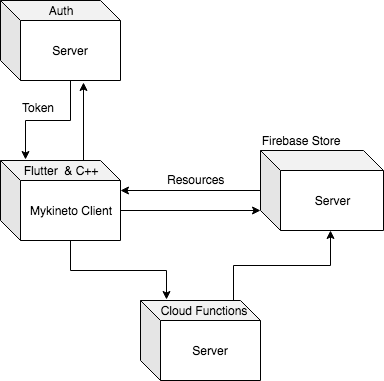
\includegraphics[scale=0.7]{fig/client-server.png}}  
	\caption{Deployment diagram}
	\label{fig:uml-client-server}
\end{figure}

% Scopul este dea a motiva pacientul prin raporte zilnice cu activitatea lui.
% In acest sens se va rula in timp real algoritmi de pose estimation pe imaginile reciptionate 
% de la camera telefonului mobil si vom salva datele generate in firebase.
The goal is to motivate the patient through daily reports with his or her work.
In this case, real-time estimation algorithms will be run on the images received from the mobile phone camera and we will save the data generated in firebase.

% In Figura \ref{fig:uml-mobile} putem observa modul in care se salveaza datele obtinute de la algoritmul de pose estimation.
In Figure \ref{fig:uml-mobile}, we can see how the data obtained from the pose estimation algorithm is saved.

% Astfel de fiecare daca cand incepem sa facem un exercitiu se creata o noua sessiune in care se vor salvate toate miscarile detectate de algoritmul, in timp ce facem exercitul.
So, each time we start an exercise, we create a new session that will save all the movements detected by the algorithm while doing the exercise.

 \begin{figure}[htbp]
	\centerline{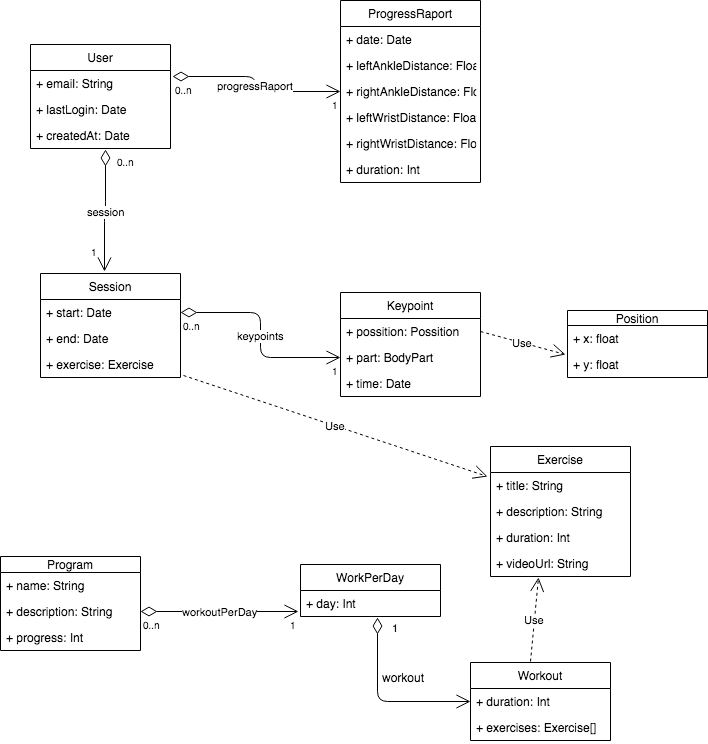
\includegraphics[scale=0.6]{fig/uml-mobile.png}}  
	\caption{Class diagram with mobile application architecture}
	\label{fig:uml-mobile}
\end{figure}

% Pentru detectarea vom folosi o reata neuronala de convolutie cu o arhitectura specializata in estimarea posturilor.
For detection, we will use a convolution neural network with a specialty architecture for pose estimation.
% Arhitectura retelei este descrisa in articolul "Convolutional pose machine" \cite{DBLP:journals/corr/WeiRKS16}.
The architecture of the network is described in the article "Convolutional pose machine" \cite{DBLP:journals/corr/WeiRKS16}.

% Acesta retea a fost implementat in python folosind libraria tensorflow. Dupa antrenarea ei am obtinut un model care a fost convertit in unul optimizat pentru a rula pe dispozitive mobile, numit tensorflow lite.
% Dupa testarea lui sa constat ca performantele sunt slabe datorita rulari lui pe CPU.
This network was implemented in python using the tensorflow library. After training, I got a model that was converted into an optimized one to run on mobile devices, called tensorflow lite.
After testing it was found that the performance is weak due to its running on the CPU.

% Dupa un research am descoperit o librarie care stie sa convertesca modelul tensorflow lite intr-un model capabil sa folosesca placa grafica. Acesta librarie se numeste Mobile AI Compute Engine (MACE)  care a fost dezvoltata de cei de la XiaoMi. Pentru a putea folosi MACE a trebui sa integram o legatura dintre android si C++, deoarece macea este scris in C++ folosind Android NDK.
After a research we found a library that knows how to convert the tensorflow lite model into a model capable of using the graphics card. This framework is called the Mobile AI Compute Engine (MACE), that was developed by XiaoMi. To be able to use MACE, I have to integrate a connection between android and C ++, because the MACE is written in C ++, we will use Android NDK for integration.

% In urma integrari sa obtinut performate mult mai bune, ajungand la 30-40 de framuri pe secunda.
% Obinund o rularea a modelului in 17 ms.
Following integration, much better performances were achieved, reaching 30-40 frames per second. Obtain a run of the model in 30-40 ms on the image.

% Mai sus am descris cum se salveaza sesiuni in timp ce utilizatorul face exerciti.
% Pe baza acestor sesiuni se vor genera raporte. Astfel se foloseste un cloud function care ia toate sesiunile din ziua curenta si genereaza un ProgressReport, conform diagramei din Figura \ref{fig:uml-mobile}.
Above we described how to save sessions while the user is doing exercises.
Based on these sessions, reports will be generated. This makes use of a cloud function that takes all sessions of the current day and generates a ProgressReport, according to the diagram in Figure \ref{fig:uml-mobile}.
% In urmatorul capitol vom da mai multe detali legate de implementarea aplicatie.
In the next chapter we will give you more details about the implementation of the application.

\subsection{Implementation}
% Pentru implementarea aplicatie sa folosit Flutter.
% Flutter este un framework facut de cei de la google, este scris in limbajul de programare Dart. Permitea rularea aceluias cod pe mobile, desktop, web si dispozitive IoT. Acesta este orientat pe componente oferind o reutilizarea a codului crescuta.
Flutter was used to implement the application.
Flutter is a framework made by google, is written in Dart programming language. It allowed running the same code on mobile, desktop, web and IoT devices. It is component-oriented offering a reuse of increased code.

% Daca am face o comparatie in Flutter si React Native putem observa ca din punct de vedere arhitectural ambele implementeaza concepte asemanatoare, cum ar fi componentele, provider consumer, arhitectura de Flux.
If we make a comparison between Flutter and React Native, we can see that architecturally both implement similar concepts, such as components, provider-consumer, Flux architecture.
% Dar mare diferenta consta in implementarea interna.
% React native foloseste componente native de android, prin folosirea unui cancal de comunicare pentru componenta din javascript si cea native.
% Flutter a renuntat la acesta idee , nu mai folosind componente native, a recurs la desenarea acestora direct prin utilizarea API internat care defapt il folosesc si componentele native pentru a fi desenate pe UI.

But the big difference is the internal implementation.
React native uses native Android components by using a communication channel for the javascript and native component.
Flutter gave up this idea, no longer using native components, resorted to drawing them directly using the board API that actually uses native components to draw on the UI.
%  \begin{figure}[htbp]
% 	\centerline{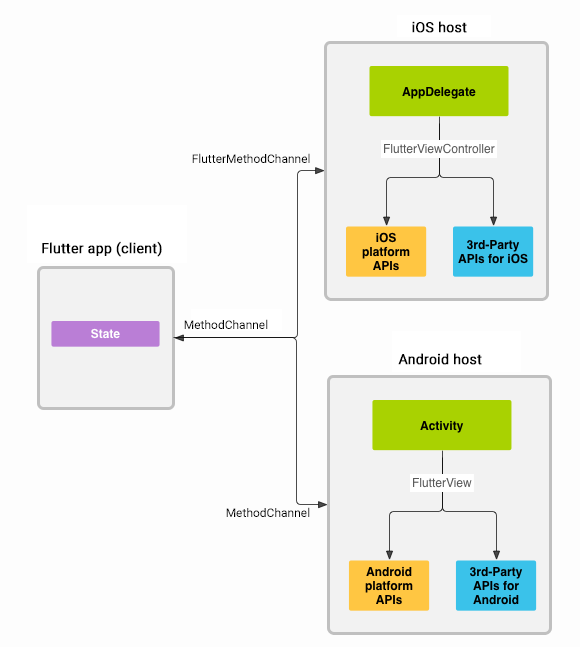
\includegraphics[scale=0.7]{fig/PlatformChannels.png}}  
% 	\caption{Architectural - Platform channels \cite{flutter}}
% 	\label{fig:flutter-plaform-channels}
% \end{figure}

% Ca sa integram partea de pose estimation a fost nevoie de a deschide un activity din android folosindune de arhitectura Flutter care permite comunicare dintre codul scris in dart cu cel scris in java.
In order to integrate the pose estimation part it was necessary to open an activity from android using the Flutter architecture that allows communication between the written code in the Dart with the one written in Java.

% Pentru a obtine performante mari ale algoritmului de pose estimation, am folosit MACE care vine cu o metoda de a converti modelul din tensorflow intr-un model care poate rula pe placa grafica a telefonului.
To achieve high performance of the pose estimation algorithm, we used MACE that comes with a method to convert the tensorflow model into a model that can run on the graphics card of the phone.
% Ca sa desenam scheletul obtinut de algoritm vom folosi opencv, care la fel va fi integrat din C++.
To draw the skeleton obtained by the algorithm we will use opencv, which will also be integrated from C ++.

% Ca sa generam rapoarte vom rula un cloud function care va prea datele de la fiecare sesiune de exerciti si le va procesa pentru a obtine distantele parcurse. Acesta functie va crea obiecte de tipul ProgressRaport, se pot observa in Figura 2.
In order to generate reports, we will run a cloud function that will also take the data from each exercise session and process them to get the distance traveled. This function will create ProgressRaport objects, as can be seen in Figure \ref{fig:uml-mobile}.

% Acesta distanta va fi calculata cu ajutorul formulei matematice a distantei euclidiane.
% Astfel vom parcurge tot cate doua detectie de cordonate  si vom calcula distanta din ele. Algoritmul va exclude distantele foarte mici pentru a scadea erroare.
This distance will be calculated using the mathematical formula of the Euclidean distance.
So we'll take two coordinate detections and calculate the distance from them. The algorithm will exclude very small distances to lower the error.


\subsection{User manual}



% Aplicația este disponibilă momentan doar pentru
% sistemele de operare android, chiar dacă varianta finală este
% cross-platform, fiind disponibilă și în varianta iOS, din cauza
% lipsei unui telefon cu sistem de operare iOS, nu putem garant
% buna funcționare a aplicatie. O puțeti descărca pe Google Play
% la acest link:https://play.google.com/store/apps/details?id=com.mykineto
% sau o puteți să folosiți apk de pe CD atașat lucrări.
The application is currently only available for
android operating systems, even if the final version is
cross-platform, also available in iOS because of
the lack of an iOS phone, we can not guarantee
good operation of the application. 

One can download on Google Play
at this link: https://play.google.com/store/apps/details?id=com.mykineto
or you can use it apk from CD attached works.

\begin{figure}[!htb]
  \centering
<<<<<<< HEAD
  \subfloat[Login]{%
    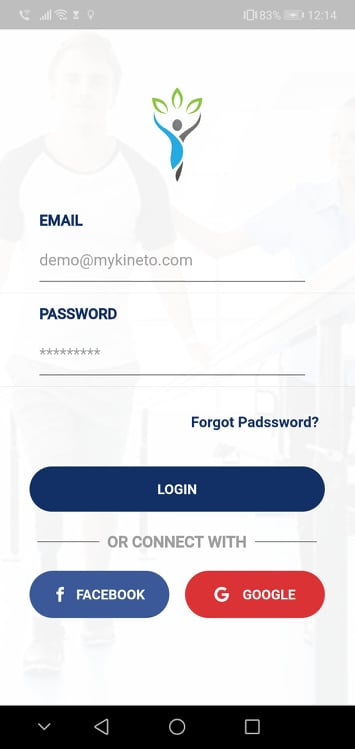
\includegraphics[width=0.3\textwidth,height=0.55\textwidth]{fig/screen-login.jpg}\label{fig:screen-login}}
  \hfill
  \subfloat[Rehab program]{%
    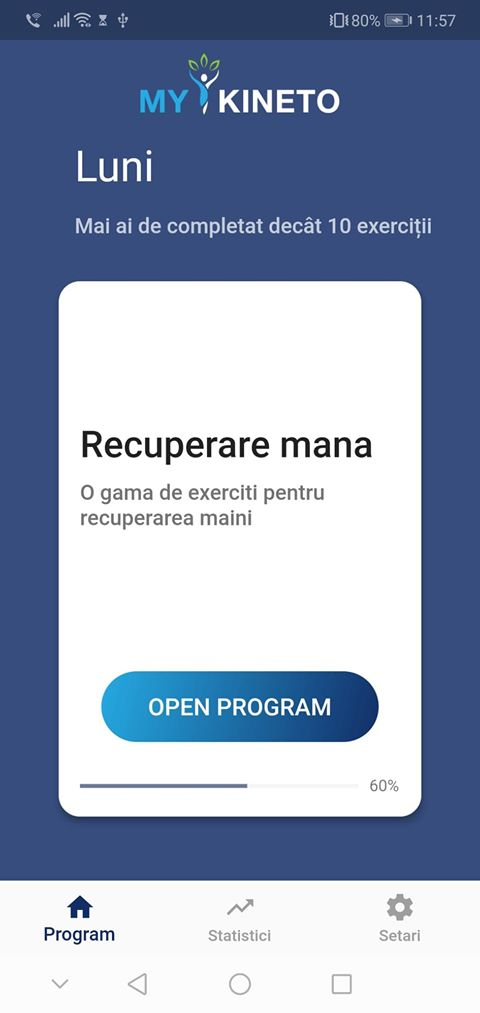
\includegraphics[width=0.3\textwidth,height=0.55\textwidth]{fig/screen-program.jpg}\label{fig:screen-program}}
=======
  \subfloat[Login\label{fig:screen-login}]{
    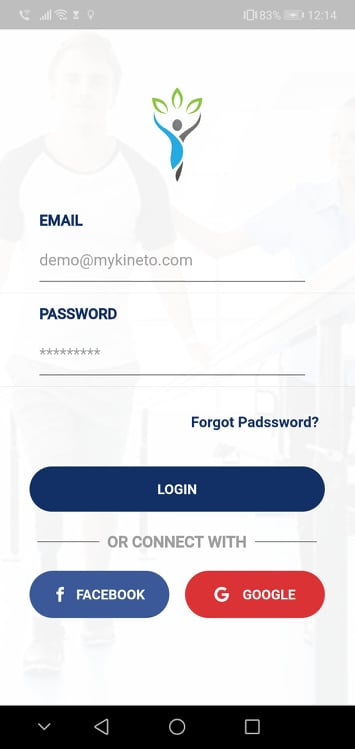
\includegraphics[width=0.3\textwidth,height=0.55\textwidth]{fig/screen-login.jpg}}
  \hfill
  \subfloat[Rehab program\label{fig:screen-program}]{
    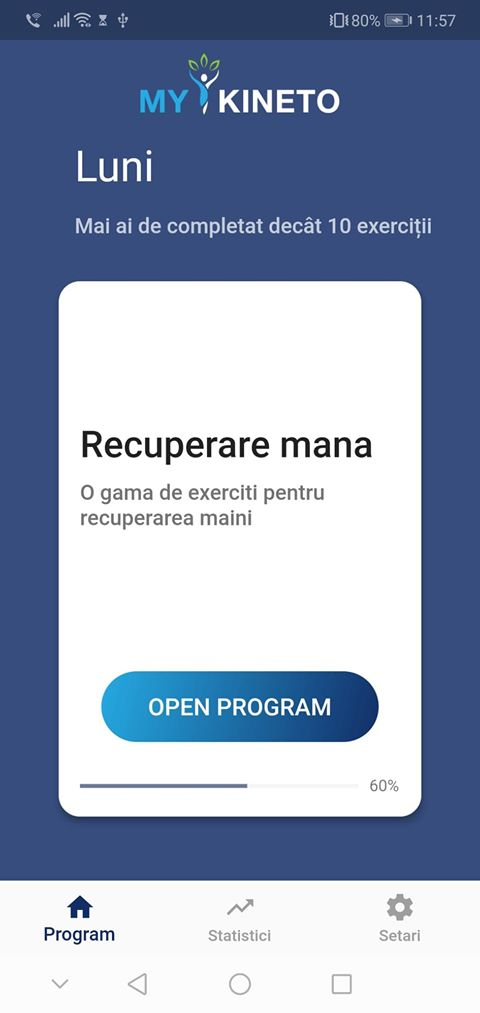
\includegraphics[width=0.3\textwidth,height=0.55\textwidth]{fig/screen-program.jpg}}
    
>>>>>>> fbad53f39a03c91483a7ea75d91c939b9c8b6f1b
    \caption{Screen with login and rehab program}
\end{figure}


% Pentru rularea aplicației aveți nevoie de un telefon cu
% sistemul de operate android la versiune minimă 9.
You need a phone to run the application that has 
android operating system with a minimal version 9.

% O să apară fereastra din Figura \ref{fig:screen-login}.
% Utilizatorul se va autentifica in aplicatie, dupa care va vedea o lista de cu programe de recuperare.
% Va intra pe un program de recuperare unde va isi va alege ziua in care va efectua exercitul.
The window in Figure \ref{fig:screen-login} will appear.
The user will login to the application and then see a list of recovery programs.
He will enter a recovery program where he will choose his day of exercise.

\begin{figure}[!htb]
  \centering
  \subfloat[Workout]{
    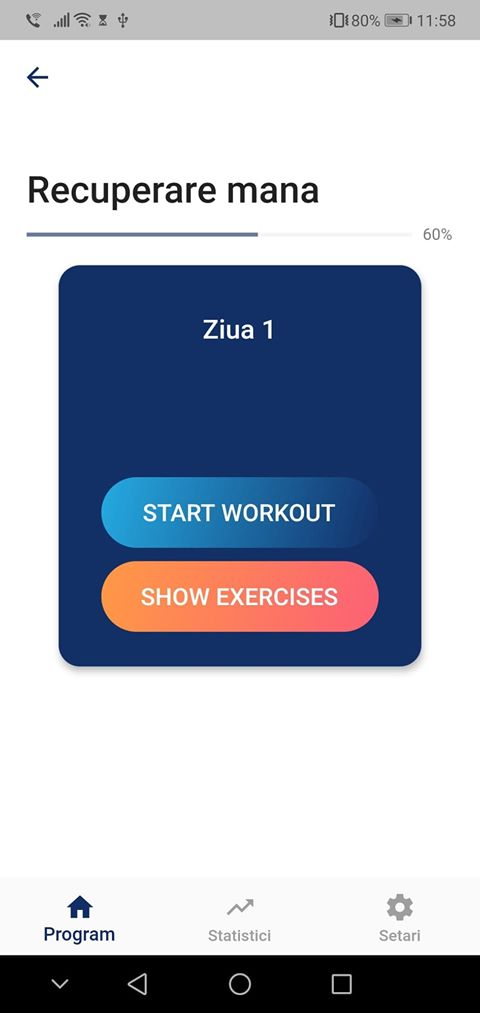
\includegraphics[width=0.3\textwidth,height=0.55\textwidth]{fig/screen-workout.jpg}\label{fig:screen-workout}}
  \hfill
  \subfloat[Exercise]{
    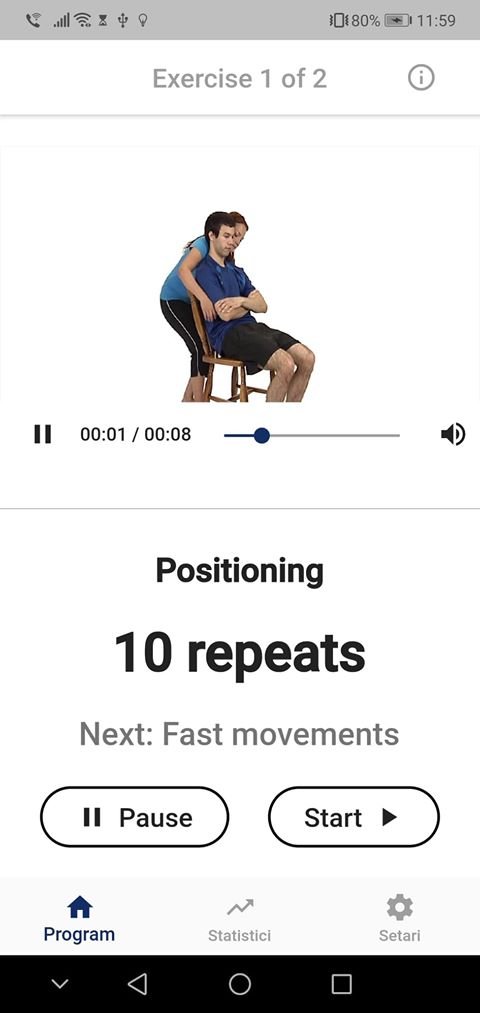
\includegraphics[width=0.3\textwidth,height=0.55\textwidth]{fig/screen-exercise.jpg}\label{fig:screen-exercise}}
    
    \caption{Screen with workout and exercise}
\end{figure}

% Dupa alegerea zilei, utilizatorul va incepe sa faca exercitiile in fata camerai video a telefonului.
% Aplicatia va monitoriza si salva miscarile facute de utilizator in timpul fiecarui exercitiu.
After selecting the day, the user will start exercising in front of the video camera of the phone.
The application will monitor and save the movements made by the user during each exercise.
\begin{figure}[!htb]
  \centering
  \subfloat[Pose Estimation]{
    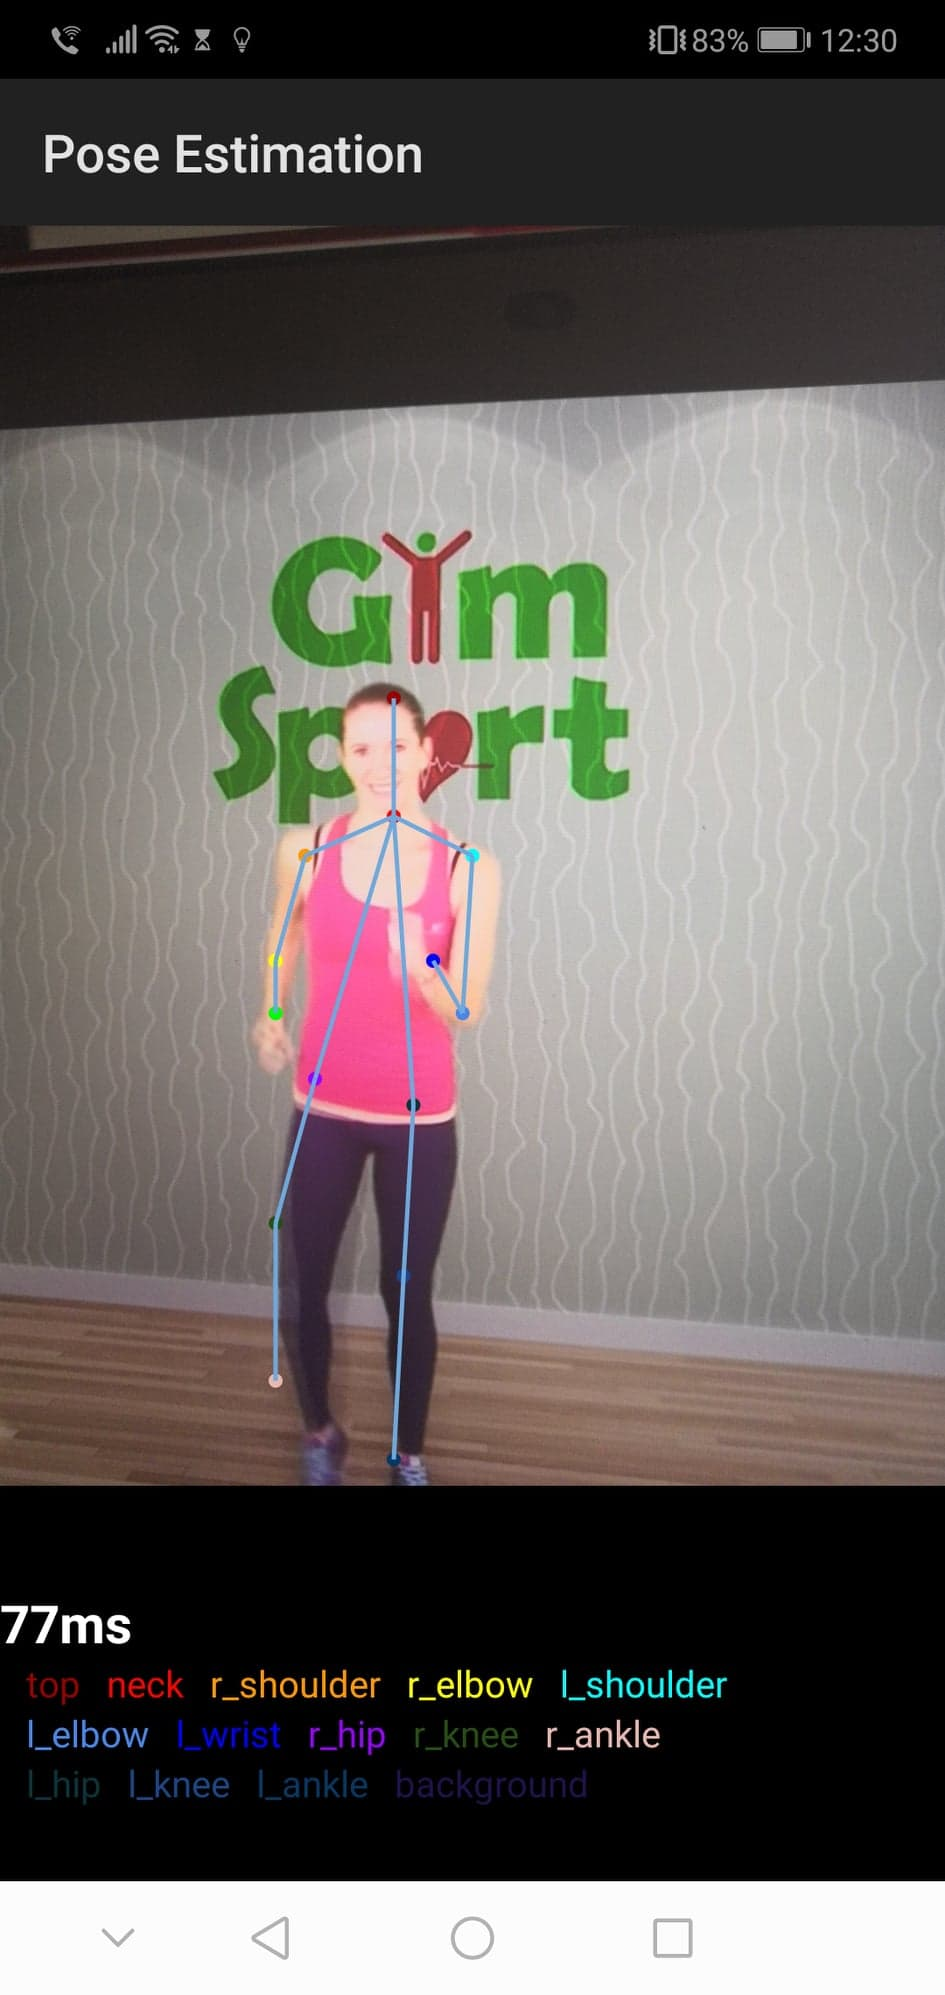
\includegraphics[width=0.3\textwidth,height=0.55\textwidth]{fig/screen-pose.jpg}\label{fig:screen-pose}}
  \hfill
  \subfloat[Statistics]{
    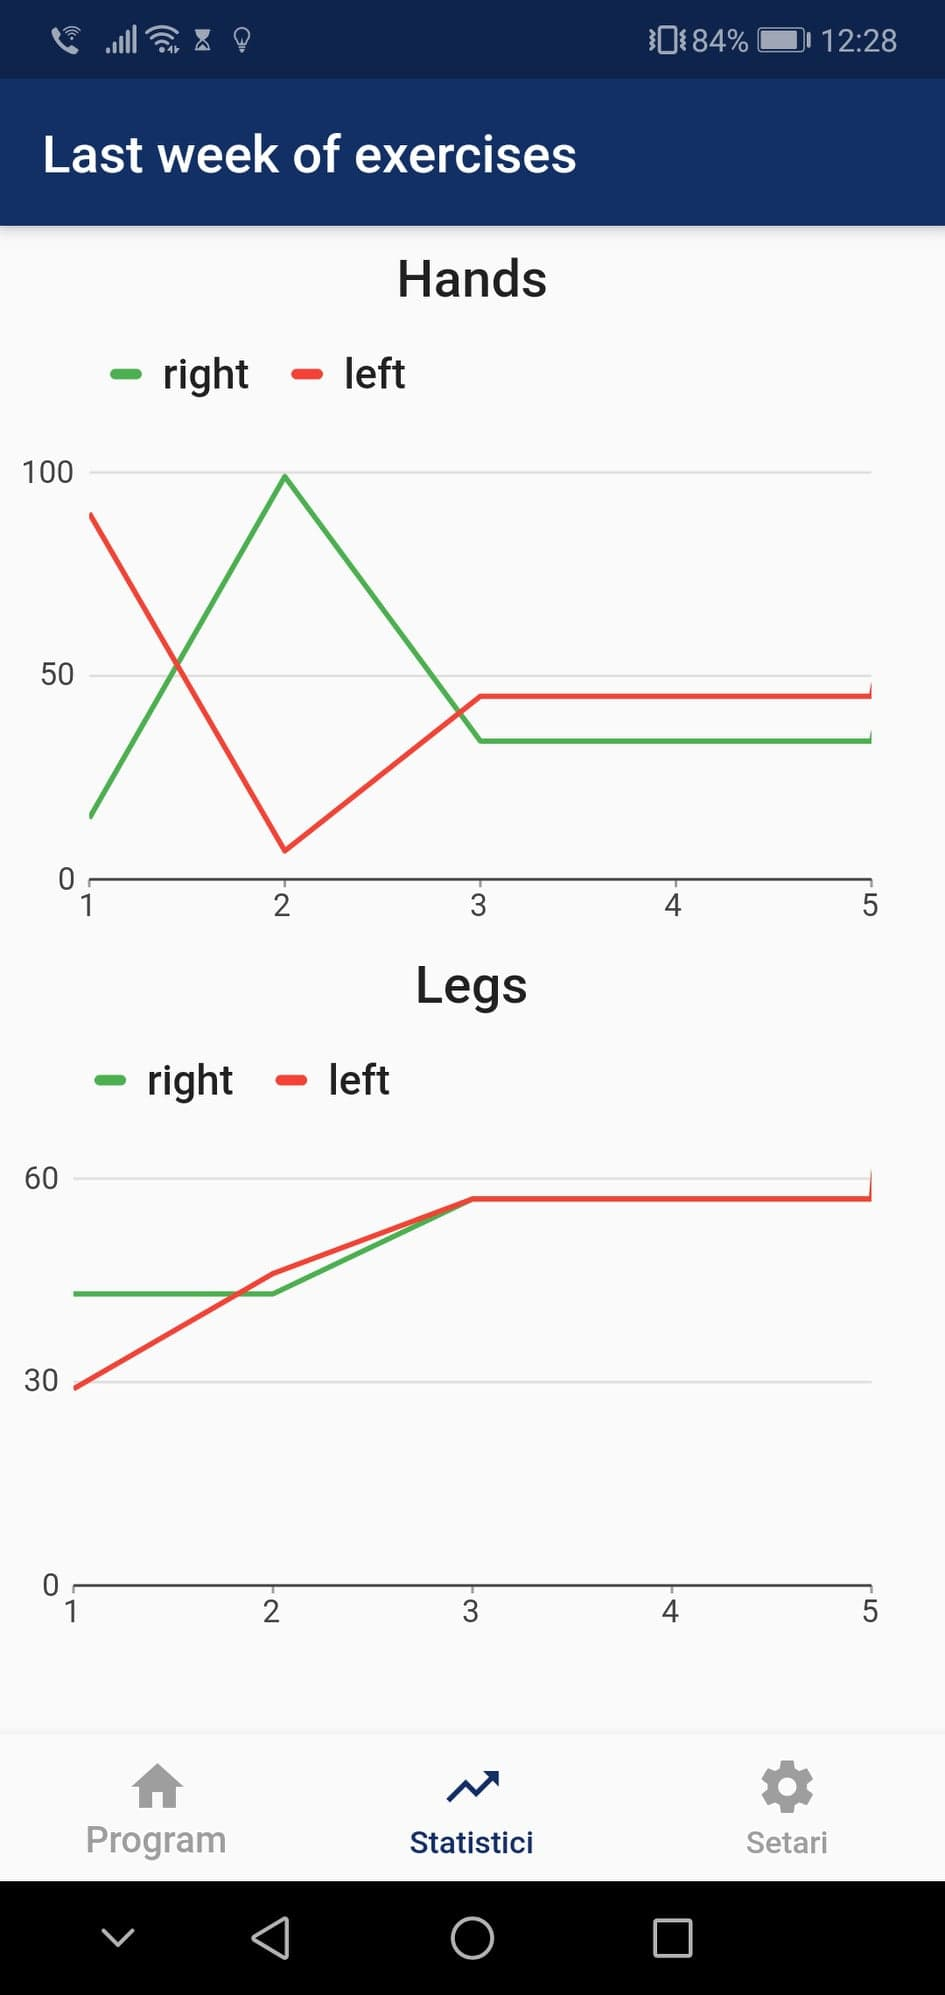
\includegraphics[width=0.3\textwidth,height=0.55\textwidth]{fig/screen-progress.jpg}\label{fig:screen-progress}}
    
    \caption{Screen with pose estimation and progress}
\end{figure}
% Utilizatorul va putea vizualiza statisticile pe zile a progresului facut de in el timpul antrenamentului.
The user will be able to view the daily statistics of the progress made during the training.

\section{Web - Application development}

% In acest capitol vom descrie modul in care a fost dezvoltat aplicatia suprinzand principale algoritmi folosinti. 
% Continund cu detalile de implementare care au contribuit la acesta aplicatie.
In this chapter we will describe how the application was developed, surprising the main algorithms used.
Continue with the implementation details that contributed to this application.


\subsection{Specification of the problem}

Application is an interactive software destined for patients who need physiotherapy
treatments. Our application guide patient to see how they need to make their exercises in 
a correct manner by showing Range of Motion (ROM) in real time and after allowing us to 
 count the number of movements. 
 
It is based on exercices, because we think that a constant and correct number of movements could be more efficient for patients then just to present them what exercices they need to do. In this manner the application guides each patient during the period they need to follow their treatment. 

\subsection{Analysis and design}

% Aplicatia va rula in browser folosind camera web pentru a detecta in real-time postura pacientului.
% Oferindune cordonatele (x, y) ale  partilor corpului pe baza carora vom aplica algoritmul de calculare a unghiurilor, obtinand astfel range of motion. 
The application will run in the browser using the webcam to detect the patient's posture in real-time.
Offering the $(x, y)$ coordinate of the body parts on which we will apply the algorithm for calculating the angles, thus obtaining a range of motion.

% In acest sens vom folosit tensorflow.js care permite rularea in browser a algoritmului de inteligenta artificiala.
% Noi vom folosi modelul PoseNet.
In this sense, we will use tensorflow.js to run the artificial intelligence algorithm in the browser.
We will use the PoseNet.

% PoseNet este un model antrenare care are la baza o reatea neuronale de convolutie, invatata sa clasifice partile corpului dand ca rezultat cordonatele acestora. In figura \ref{fig:uml-posenet} se poate observa o diagrama care prezinta structura datelor de iesire care le ofera PoseNet.
PoseNet is a training model based on a convolutional neural network, learn to classify body parts, resulting in their coordinates. Figure \ref{fig:uml-posenet} show a diagram that represent the structure of output data provided by PoseNet.

 \begin{figure}[htbp]
	\centerline{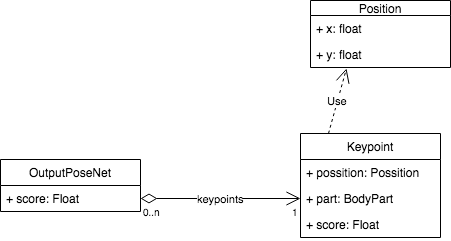
\includegraphics[scale=0.7]{fig/uml-posenet.png}}  
	\caption{PoseNet Output}
	\label{fig:uml-posenet}
\end{figure}

% PoseNet a fost realizat de cei de la google si foloseste o arhitectura de tip MobileNet.
% MobileNet este o arhitectura optimizata pentru a rula pe dispozitive cu putere scazuta de calcul, ca telefoanele.
PoseNet was developed by Google and uses a MobileNet architecture.
MobileNet is an optimized architecture to run on low-power devices such as phones.

% In articolul "Mobilenets: Efficient convolutional  neuralnetworks for mobile vision applications"  \cite{DBLP:journals/corr/HowardZCKWWAA17} sunt descrise principale optimizare aduse de arhitectura numit MobileNet.
In the article "Mobilenets: Efficient convolutional neuralnetworks for mobile vision applications"  \cite{DBLP:journals/corr/HowardZCKWWAA17} are described the main optimization brought by the architecture called MobileNet.

% Cea mai importanta optimizare de performanta a fost realizata prin introducerea unui nou tip de strat, numit Depthwise Separable Convolution. Acest strat inlocuieste convolutila standard. Si mare diferenta este ca a impartit in doi pasi separati, aplicarea filtrari si combinarea.
The most important performance optimization was achieved by introducing a new type of layer, called Depthwise Separable Convolution. This layer replaces standard convolution and the big difference is that it is divide into two separate steps, applying filtration and combining.

% Pe baza keypoints obtinute de la PoseNet vom desena unghiurile dintre membrele pacientului folosind canvas.
Based on keypoints from PoseNet we will draw angles between the patient's body limbs using canvas.
% Unghiul dintre doua drepte va fi calculat folosind formula matematica, reprezentand range of motion.
The angle between two straight lines will be calculated using the mathematical formula representing range of motion.

% Pentru a numara numarul de exercitii corecte vom folosi un algoritm bazat pe unghiuri pentru fiecare tip de exercitiu.
To count the number of correct exercises we will use an algorithm based on angles for each type of exercise.

% De exemplu daca se fac squats atunci algoritmul va functiona pe baza de stari, astfel vom avea starile:
For example, if the user does the squat exercise, then the algorithm will work on states, so we will have the states:
\begin{itemize}
    % \item Inceputul exercitiului daca unghiul de la genunchi este intre 10 si 75 de grade
    \item The beginning of the exercise if the knee angle is between 10 and 75 degrees
    % \item Sfarsitul exercitiului daca unghiul de la genunchi este intre 145 si 300 de grade
    \item End of exercise if the knee angle is between 145 and 300 degrees
\end{itemize}

% Pe baza acestor doua stari, vom numara numarul de exercitii facute corect din puncte de vedere a unghiurilor.
Based on these two states, we counted the number of exercises done correctly in terms of angles.

 \begin{figure}[htbp]
	\centerline{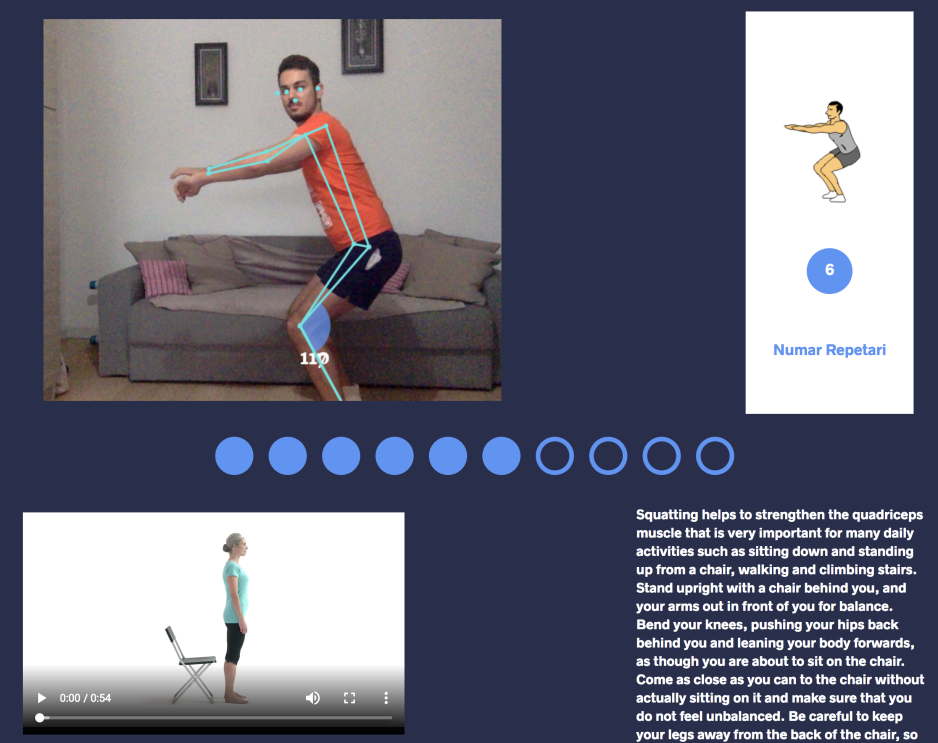
\includegraphics[scale=0.7]{fig/demo-mykineto.png}}  
	\caption{Demo MyKineto}
	\label{fig:demo-web-mykineto}
\end{figure}

% In Figura \ref{fig:demo-web-mykineto} se poate vedea cum algoritmul numara numarul de repetari corecte si afiseaza punctele detectate in timp real de algoritm folosind canvas.
In Figure \ref{fig:demo-web-mykineto} we can see how the algorithm counts the number of correct iterations and displays the real-time detected algorithm points using canvas.


\subsection{Implementation}

% Pentru implementarea acestei aplicatie web sa folosit react in dezvoltarea interfetei grafice.
% Iar pe partea de pose estimation am folosit tensorflow.js impreuna cu modelul PoseNet.
To implement this web application, React.js was used in the development of the graphical interface.
And on the estimation pose we used Tensorflow.js along with the PoseNet model.

% Ce este React? React este o bibliotecă JavaScript folosită în dezvoltarea interfețelor web.
% Prima versiune a fost lansată de către facebook în Martie 2013. Față de alte platforme React vine cu
% capacitatea sa de a fi declarativ, bazat pe componente și faptul că este reutilizabil \cite{fb-react}.
What is React? React is a JavaScript library used to develop web interfaces.
The first version was released by facebook in March 2013. Faced with other platforms React comes with
its ability to be declarative, component-based, and reusable \cite{fb-react}.

% Biblioteca React permite crearea de componente pentru fiecare stare a aplicației, în cazul
% modificări unei stări se vor randa componentele care trebuie să apară în cazul acelei stări, astfel se
% crește performanța aplicației.
The React Library allows you to create components for each application status, changing the status of the components to occur for that state, and thus increasing the performance of the application.

% React folosește noua sintaxă JavaScript Extension (JSX) care este asemănătoare cu sintaxa
% Hypertext Markup Language (HTML), defirența este că pe post de marcatori putem folosi
% componente React \cite{jsx-react}.

React uses the new JavaScript Extension (JSX) syntax that is similar to the Hypertext Markup Language (HTML) syntax, the difference is that as markers we can use react components \cite{jsx-react}.

% O cauză a modelului declarativ bazat pe componente constă în reutilizarea codului, fiecare
% componentă își încapsulează și gestionează propria stare. Se pot realiza interfețe complexe prin
% asamblarea lor precum niște pazăluri. Fiecare componentă își gestionează starea curenta, acesta find un task dificil în realizarea unor arhitecturi complexe.
A cause of the component-based declarative model is the reuse of the code, each component encapsulates and manages its own state. Complex interfaces can be made by assembling them like puzzles. Each component manages its current state, which is a difficult task in building complex architectures.

% Pentru o eficiență mai sporită, React folosește Virtual DOM, care este o abstractizare a
% DOM, fiindcă operațiile asupra DOM sunt încete \cite{virtual-dom-react}.
For greater efficiency, React uses Virtual DOM, which is an abstraction of DOM, because DOM operations are slow \cite{virtual-dom-react}.

% Tensorflow.js permite rula algoritmilor de inteligenta artificala in mediul javascript.
% Dupa cum stim algoritmi de inteligenta artificiala, mai ales cei aplicati pe imagini sau video au nevoie de o putea mare de calcul.
Tensorflow.js allows the artificial intelligence algorithms to run in javascript.
As we know artificial intelligence algorithms, especially those applied to images or video need a high performance of computing.
% Pentru a rezolva aceasta problema, tensorflow.js ruleaza algoritmi folosind WebGL in mod automat.
% Acest lucra face ca algoritmi sa ruleze pe GPU \cite{tensorflow.js}.
To solve this problem, tensorflow.js runs algorithms using WebGL automatically.
This work makes algorithms run on the GPU \cite{tensorflow.js}.

% Pe lângă asta, pentru dezvoltarea aplicație s-a folosit typescript care este un super set tipizat a lui javascript și mediul de dezvoltare Visual Studio Code.
Additionally, for the development of the application we used a typescript what is a superset of JavaScript which primarily provides optional static typing, classes and interfaces. Also we use the Visual Studio Code development environment.

\section{Experimental results}

% In urma implementari celor doua variante de mai sus am facute mai multe teste legate de performanta algoritmilor.
Following the implementation of the above two variants we performed several tests related to the performance of the algorithms.
% Mai exact, cat de repede ruleaza algoritmul de pose estimation pe o imagine. Cu cat ruleaza mai repede cu atata avem p performanta mai buna, targetul nostru find de 30 frame per seconds.
Specifically, how fast the estimation pose algorithm runs on an image. The faster it runs, the better our performance will become and our target is to obtain 30 frames per second.

 \begin{figure}[htbp]
	\centerline{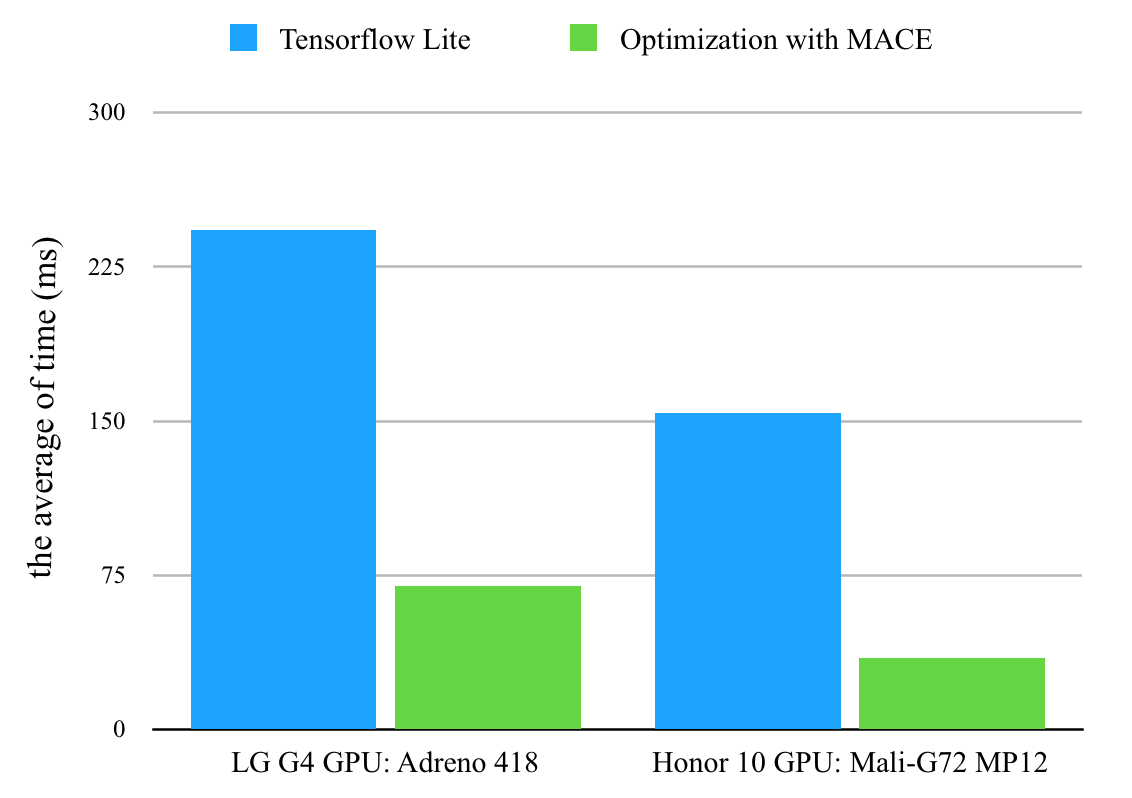
\includegraphics[scale=0.7]{fig/mobile-performace.png}}  
	\caption{The performance of the pose estimation algorithm run on two devices with optimized and non-optimized model.}
	\label{fig:mobile-perf}
\end{figure}

% In Figura \ref{fig:mobile-perf} putem observa o create cu 50\% a performantei in cazul modelul optimizat pentru aplicatie mobila.
In Figure \ref{fig:mobile-perf} we can see a 50\% increase performance for the mobile optimized model.

% In cazul aplicatie web, lucrurile stau un pic diferit. Am incerc sa fac o comparatie intre rularea algoritmului pe client sau pe server. Se poate observa clar din figura \ref{fig:web-perf} ca varianta cu folosirea unui servarul se exclude doarece ori cat ar fi servarul de bun durata requestului dureaza in medie 50 ms doarece se trimit un numar mare de date.
In case of a web application, things are a bit different. I'm trying to make a comparison between running the algorithm on the client or on the server. It can be clearly seen from Figure \ref{fig:mobile-perf} that the version with using the server is excluded because the duration of the request lasts for an average of 50 ms since a large number of data is sent.

 \begin{figure}[htbp]
	\centerline{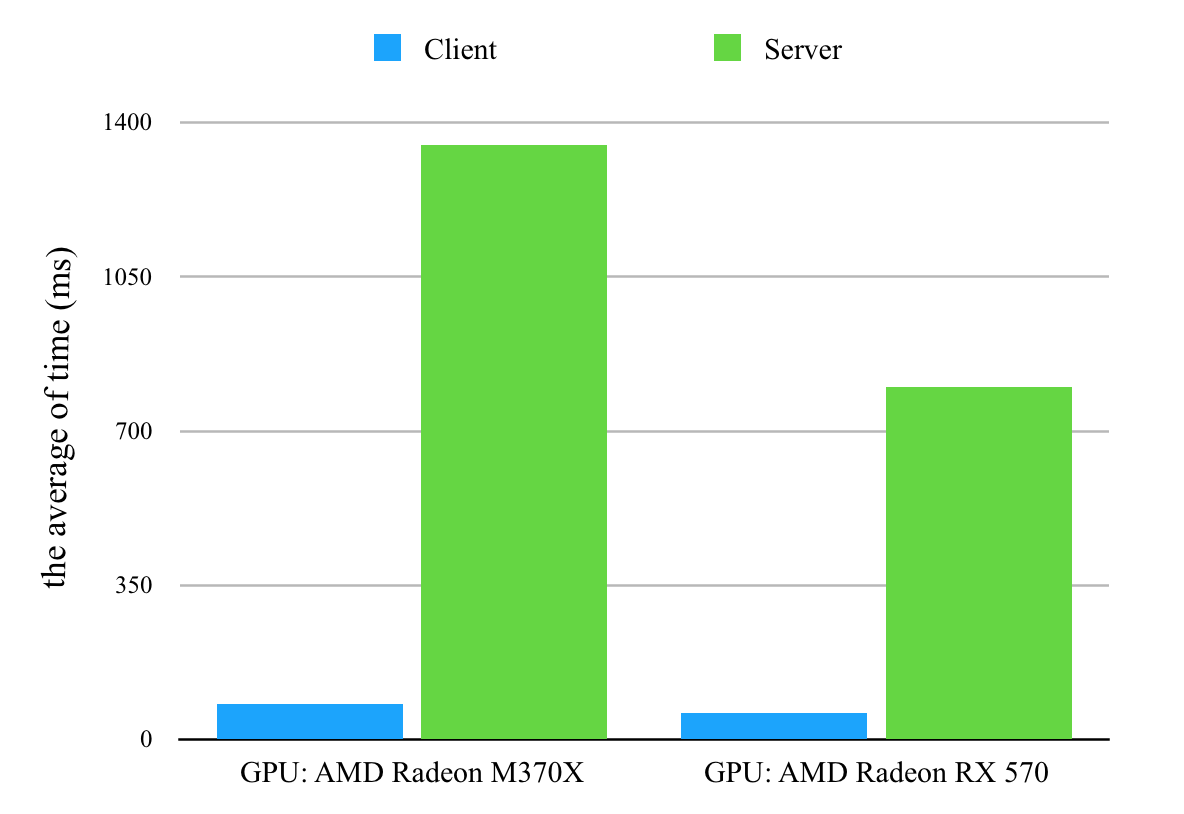
\includegraphics[scale=0.7]{fig/web-performace.png}}  
	\caption{The performance of the pose estimation algorithm run on web}
	\label{fig:web-perf}
\end{figure}

\section{Possible extensions}

% O posibila extindere a sistemului ar consta in unificarea celor doua aplicatie astfel incat sa avem cele doua variante prin care motivam pacientul.Varianta prin care urmarim progresul prin calcul distantelor si varinata in care calculam range of motion , numarand numarul de exerciti corecte. 
% Sa fie disponibile atata pe web cat si pe mobile.
A possible extension of the system would be to unify the two applications so that we have the two variants by which we motivate the patient. The variant which we follow the progress by calculating the distances and the variant in which we calculate the range of motion, counting the number of correct exercises.
Both will be available on the web and on the mobile.

% In plus ne gandim la o extindere a functionalitati incat sa acoperim scenarile de utilizare minimale pentru un utilizator care are probleme de sanatate. In primul rand ar trebui implementate comenzile vocale.
In addition, we are considering extending functionality to cover minimal usage scenarios for a user who has health problems. First of all, voice commands should be implemented.
% Ar fi de interes implementare unui model pentru fizioterapeut, prin care el sa gestioneze programul de recuperare a fiecarui pacient plus accesul pe raportele cu performantele lui.

It would be of interest to implement a model for a physiotherapist to manage each patient's recovery program plus access to performance reports.

% O alta optimizare care o vad este combinarea celor doua arhitecturi de retele neuronale in una singura.
% Astfel oferind o posibila de imbunatatire a performantei. Dar si gasirea unei configuratie optima de retea care sa functioneze atata pe web cat si pe mobile.
Another optimization that I see is the combination of the two neural network architectures into one.
This provides the possibility of increasing the performance. And finding an optimal network configuration that works both on the web and on the mobile.
% Tot la optimarea ne puteam gandi la implementarea unui algoritm de urmarirea a contururilor. Astfel detectia facanduse doar la inceput. 

At optimization we can also think of implementing a tracking algorithm based on contour. The detection will always be at the beginning.

% Dupa ne inspiram de la concurenta, am putea implementa un joc in care pacientul este pus sa faca anumite  miscari pentru a castig a jocul.
After inspiring us from the competition, we could implement a game in which the patient have to do  certain moves to win the game.